\documentclass[12pt, a4paper]{book}

% Core packages
%% Preamble
\usepackage{blindtext}

% Core
\usepackage[utf8]{inputenc}
\usepackage[american, spanish, es-tabla]{babel}
\usepackage{hyperref}
\usepackage{bookmark}
\usepackage{emptypage}

% Graphics
\usepackage{pdfpages}
\usepackage{graphicx}
\usepackage{epsfig}

% Bibliography
\usepackage[autostyle]{csquotes}
\usepackage[bibstyle=science, 
			citestyle=authoryear, 
            sorting=none, 
            autopunct=false,
            uniquename=init, 
            maxbibnames=4,
            articletitle=true]{biblatex}
\addbibresource{references.bib}
\AtEveryCite{\color{blue}}
\DefineBibliographyStrings{spanish}{
  presentedat = {presentado en~}
}

% Fancy header and footer
\usepackage{fancyvrb}
\usepackage{fancyhdr}

\fancypagestyle{onlyfooter}
{
    \renewcommand{\headrulewidth}{0pt}
    \fancyfoot[C]{\thepage}
    \fancyhead{}
}

\pagestyle{fancy}
\setlength{\headheight}{20pt}
\fancyfoot[C]{\thepage}
\fancyhead[LE,RO]{\leftmark}
\fancyhead[RE,LO]{}

% Appendix
\usepackage[titletoc]{appendix}

%%%%% Tweaks %%%%%
% Small captions size
\usepackage[font=small]{caption}

% Don't indent paragraphs.
\usepackage{parskip}
\setlength\parindent{0em}

% Reduce spacing before/after subsubsection
\usepackage{titlesec}
\titlespacing*{\subsection}{0pt}{2.25ex plus 1ex minus .2ex}{0.1ex plus .2ex minus .2ex}
\titleformat{\chapter}[display]
  {\bfseries\Large}
  {\filright\MakeUppercase{\chaptertitlename} \Huge\thechapter}
  {1ex}
  {\titlerule\vspace{1ex}\filleft}
  [\vspace{1ex}\titlerule]

\usepackage{tikz}
\usetikzlibrary{shapes, arrows, positioning, fit, babel}

\usepackage{algorithm}
\usepackage{algpseudocode}
\makeatletter\renewcommand{\ALG@name}{Algoritmo}

\usepackage{textcomp}
\usepackage{longtable}

\usepackage{listings}

\def\verbatim@font{\linespread{1}\normalfont\ttfamily}


% Важно: для minted требуется компиляция с флагом --shell-escape
% pdflatex -shell-escape <file>.tex
% For minted (method 1)
\usepackage{minted}

% For tcolorbox (method 2)
%\usepackage[most]{tcolorbox}
% \tcbuselibrary{listingsutf8}

% For listings (method 3)
% already included

% For fancyvrb (method 4)
%\usepackage{fancyvrb}

% For file name headers
\newcommand{\codefileheader}[1]{\vspace{1em}\noindent\textbf{File:}~\texttt{#1}\par\vspace{0.5em}}


% Load variables
\def \alumno {Donat Shergalis}
\def \tutor {Gabriel Jesús Luque Polo}
% \def \cotutor {Nombre del cotutor} % optional (comment if none)
\def \departamento {ESCUELA TÉCNICA SUPERIOR DE INGENIERÍA INFORMÁTICA}
\def \grado {MÁSTER UNIVERSITARIO EN INGENIERÍA DEL SOFTWARE E INTELIGENCIA ARTIFICIAL}
\def \facultad {ESCUELA TÉCNICA SUPERIOR DE INGENIERÍA INFORMÁTICA}
\def \fecha {Septiembre de 2025}
\def \tituloes {Diseño de un método comparativo para copilotos de código con IA}
\def \tituloen {Design of an Evaluation Method for AI Programming Assistants}
% \def \subtituloes {Subtítulo en ES} % optional (comment if none)
% \def \subtituloen {Subtítulo en EN} % optional (comment if none)

% Extra pages
%\def \addacknowledgments {} % optional: comment this line if you don't want to include acknowledgments
\def \addappendix {}  % optional: comment this line if you don't want to include appendix
\def \configpar {} % optional: comment this line if you don't want first-line indents in paragraphs


\begin{document}

\thispagestyle{empty}

\input{pages/01-etiqueta.tex}

\newpage\null\thispagestyle{empty}\newpage
\newpage\null\thispagestyle{empty}\newpage

\thispagestyle{empty}
\begin{center}
  \begin{figure*}[h]
    \centering
    \includegraphics[scale=0.2]{images/marcauma.png}
  \end{figure*}

  \MakeUppercase{\facultad} \\
  \MakeUppercase{\grado} \\
  \vspace{3cm}
  {\large	\tituloes} \\
  \ifdef{\subtituloes}{
    \textit{\subtituloes} \\
  }{}
  {\large	\tituloen} \\
  \ifdef{\subtituloen}{
    \textit{\subtituloen} \\
  }{}  \bigbreak
  Realizado por \\
  \textbf{\alumno} \\
  Tutorizado por \\
  \textbf{\tutor} \\
  \ifdef{\cotutor}{
    Cotutorizado por \\
    \textbf{\cotutor} \\
  }{}
  Departamento \\
  \textbf{\departamento}
  \bigbreak
  UNIVERSIDAD DE MÁLAGA \\
  MÁLAGA, \fecha
\end{center}

\vfill

Fecha defensa: \\
El Secretario del Tribunal


\newpage\null\thispagestyle{empty}\newpage

\ifdef{\addacknowledgments}{
    \pagenumbering{roman}
    \thispagestyle{onlyfooter}
    \setcounter{page}{1}
    \input{pages/03-agradecimientos.tex}
    
    \newpage\null\thispagestyle{empty}\newpage
    
    \thispagestyle{onlyfooter}
    \setcounter{page}{2}
    %\documentclass[../main.tex]{subfiles}

%\begin{document}
%% begin abstract format
\makeatletter
\renewenvironment{abstract}{%
    \if@twocolumn
      \section*{Resumen \\}%
    \else %% <- here I've removed \small
    \begin{flushright}
        {\filleft\Huge\bfseries\fontsize{48pt}{12}\selectfont Resumen\vspace{\z@}}%  %% <- here I've added the format
        \end{flushright}
      \quotation
    \fi}
    {\if@twocolumn\else\endquotation\fi}
\makeatother
%% end abstract format
\begin{abstract}
%\Blindtext

Los benchmarks juegan un papel crucial en el desarrollo, evaluación y selección de modelos para su uso práctico. Los benchmarks y frameworks existentes presentan limitaciones. Diferentes benchmarks se compensan parcialmente entre sí, pero ninguno es universal: los problemas incluyen saturación, fuga de datos, métricas y resultados limitados, y altos costos energéticos y computacionales.


Proponemos un enfoque para extraer la máxima información útil de cada ejecución de benchmark, aumentando la comprensión para investigadores y profesionales, al mismo tiempo que se reduce el impacto ambiental. Al hacer las ejecuciones más informativas, se pueden evitar repeticiones innecesarias, disminuyendo el consumo de energía. El enfoque permite la selección flexible de tareas, configuraciones detalladas e integración de múltiples criterios de evaluación en una sola ejecución. Se implementó un prototipo para demostrar la viabilidad, validar la funcionalidad y examinar las limitaciones.



\bfseries{\large{Palabras Clave:}} LLM, modelos de lenguaje grande, benchmarks, marco de evaluación, impacto ambiental, consumo de energía, saturación de benchmarks, fuga de datos, LLM-como-juez


\vspace{1cm}
\begin{center}
  \rule{0.5\textwidth}{.4pt}
\end{center}
\vspace{1cm}


\newpage
\textbf{Abstract}:

\normalfont
Benchmarks play a crucial role in developing, researching, and evaluating models for practical use. Existing benchmarks and frameworks have limitations. Different benchmarks partially compensate for each other, but none is universal: issues include saturation, data leakage, limited metrics and outputs, and high energy and computational costs.


We propose an approach to extract the maximum useful information from each benchmark run, enhancing insights for researchers and practitioners while reducing environmental impact. By making benchmark executions more informative, redundant runs can be avoided, lowering energy consumption. The approach enables flexible task selection, fine-grained configuration, and integration of multiple evaluation criteria in a single execution. A prototype was implemented to demonstrate feasibility, validate functionality, and examine limitations.

\bfseries{\large{Keywords:}} LLM, large language models, benchmarks, evaluation framework, environmental impact, energy consumption, benchmark saturation, data leakage,LLM-as-a-judge

\end{abstract}
%\end{document}
    
    \newpage\null\thispagestyle{empty}\newpage
    
    \setcounter{page}{3}
    \pagenumbering{arabic}
    \renewcommand{\contentsname}{Table of Contents}
}{
    \thispagestyle{empty}
    %\documentclass[../main.tex]{subfiles}

%\begin{document}
%% begin abstract format
\makeatletter
\renewenvironment{abstract}{%
    \if@twocolumn
      \section*{Resumen \\}%
    \else %% <- here I've removed \small
    \begin{flushright}
        {\filleft\Huge\bfseries\fontsize{48pt}{12}\selectfont Resumen\vspace{\z@}}%  %% <- here I've added the format
        \end{flushright}
      \quotation
    \fi}
    {\if@twocolumn\else\endquotation\fi}
\makeatother
%% end abstract format
\begin{abstract}
%\Blindtext

Los benchmarks juegan un papel crucial en el desarrollo, evaluación y selección de modelos para su uso práctico. Los benchmarks y frameworks existentes presentan limitaciones. Diferentes benchmarks se compensan parcialmente entre sí, pero ninguno es universal: los problemas incluyen saturación, fuga de datos, métricas y resultados limitados, y altos costos energéticos y computacionales.


Proponemos un enfoque para extraer la máxima información útil de cada ejecución de benchmark, aumentando la comprensión para investigadores y profesionales, al mismo tiempo que se reduce el impacto ambiental. Al hacer las ejecuciones más informativas, se pueden evitar repeticiones innecesarias, disminuyendo el consumo de energía. El enfoque permite la selección flexible de tareas, configuraciones detalladas e integración de múltiples criterios de evaluación en una sola ejecución. Se implementó un prototipo para demostrar la viabilidad, validar la funcionalidad y examinar las limitaciones.



\bfseries{\large{Palabras Clave:}} LLM, modelos de lenguaje grande, benchmarks, marco de evaluación, impacto ambiental, consumo de energía, saturación de benchmarks, fuga de datos, LLM-como-juez


\vspace{1cm}
\begin{center}
  \rule{0.5\textwidth}{.4pt}
\end{center}
\vspace{1cm}


\newpage
\textbf{Abstract}:

\normalfont
Benchmarks play a crucial role in developing, researching, and evaluating models for practical use. Existing benchmarks and frameworks have limitations. Different benchmarks partially compensate for each other, but none is universal: issues include saturation, data leakage, limited metrics and outputs, and high energy and computational costs.


We propose an approach to extract the maximum useful information from each benchmark run, enhancing insights for researchers and practitioners while reducing environmental impact. By making benchmark executions more informative, redundant runs can be avoided, lowering energy consumption. The approach enables flexible task selection, fine-grained configuration, and integration of multiple evaluation criteria in a single execution. A prototype was implemented to demonstrate feasibility, validate functionality, and examine limitations.

\bfseries{\large{Keywords:}} LLM, large language models, benchmarks, evaluation framework, environmental impact, energy consumption, benchmark saturation, data leakage,LLM-as-a-judge

\end{abstract}
%\end{document}
    
    \newpage\null\thispagestyle{empty}\newpage
    
    \setcounter{page}{2}
    \pagenumbering{arabic}
    \renewcommand{\contentsname}{Table of Contents}
}

\setcounter{tocdepth}{3}
\tableofcontents

\newpage\null\thispagestyle{empty}\newpage
\cleardoublepage

\ifdef{\configpar}{
    \setlength{\parindent}{10px}
}{}

\setcounter{page}{1}
% Checklist and TO DOs
% Describe metodology of the work with sources
% Classification of Benchmarks
% add Pros and Cons of my approach compared with anothers
% why do most benchmark use fixed sets of tasks
% why do we need a modular benchmark
% What do benchmarks check
  % Categories of tasks: Math, Logic, Table understanding,  Reading comprehension, Commonsense reasoning, Vision \cite{vendrow2025largelanguagemodelbenchmarks}
%
% Why did I chose Java and Spring Boot instead of Python (because Spring AI is great), and React
% Mention that I used OpenRouter, but any provided supported by Spring AI could be used
%
% Focus more on the concept of benchmarks with UI, than in the implementation

\chapter{Introduction}

% What is missing or should be improved:
% Methodology Overview: There is no brief mention of the approach or methods used in the work. Add a short paragraph summarizing the methodology (e.g., system design, implementation, evaluation).
% Нужно описать, что я нашёл и использовал уже существующие Critical Review по теме в качетсве базы для анализа существующей литературы, затем следовал ссылкам на статьи, которые мне нужны. Последний подходящий Critical Review был опубликован в середине 2024 года, так что затем я сделал поиск по статьям за 2025 года и вторую половину 2024 года по ключевым словам, связанным с Benchmarking и LLM, выбрав среди них актуальные, отвечая на вопросы исследования. Затем, на основании собранной информации, я добавил свои собственные идеи и предложения по улучшению бенчмарков.

Large Language Models (LLMs) have revolutionized software development through AI-assisted programming tools like GitHub Copilot. However, evaluating and fine-tuning these models requires extensive benchmarking, which comes at significant computational, financial, and environmental costs. Current benchmarks often contain irrelevant tasks and provide limited customization options, making them inefficient for specific use cases.

This work explores existing benchmarks for code-generating LLMs and proposes a novel approach: an easily customizable benchmarks with detailed and conveniently explorable outputs that can be tailored to specific needs while remaining cost-effective and environmentally conscious.

% Methodology Overview
This thesis began with a comprehensive literature review, using recent critical reviews as a foundation for analyzing the state of LLM benchmarking.
The review was extended by following citations to relevant articles published in late 2024 and 2025, focusing on keywords related to benchmarking and LLMs.
The findings from this literature analysis informed the design and implementation of a modular benchmarking system, which was then evaluated for efficiency, flexibility, and environmental impact.

% Research Questions
The literature review and further research were guided by the following questions:
\begin{itemize}
    \item RQ1: What are the main limitations of current LLM benchmarks for code generation?
    \item RQ2: What metrics best reflect real-world usability and code quality?
    \item RQ3: How can benchmarks be made customizable for different user needs?
    \item RQ4: What is the environmental impact of repeated benchmarking, and how can it be reduced?
\end{itemize}

% Contributions Summary
\textbf{Main contributions of this work:}
\begin{itemize}
    \item A critical analysis of existing LLM code generation benchmarks and their shortcomings.
    \item The design and implementation of a modular, customizable benchmarking framework.
    \item Integration of environmental and cost considerations into the benchmarking process.
    \item An interactive web interface for configuring benchmarks and analyzing results.
    \item Recommendations for future benchmarking practices based on empirical findings.
\end{itemize}

\section{Problem Statement}

Benchmarking LLMs for code generation is essential for both research and practice, but current approaches face critical limitations.
Most benchmarks are fixed datasets, which leads to task saturation and data leakage as models are trained on their contents.
The lack of customization prevents researchers and practitioners from focusing on tasks relevant to their use cases.
At the same time, running large benchmarks consumes significant computational resources, resulting in high costs and environmental impact. Furthermore, benchmark outputs are often limited to single numeric metrics, which fail to capture nuanced aspects of model performance such as efficiency, style, or error patterns.

Therefore, the problem addressed in this thesis is the absence of a flexible, customizable, and sustainable benchmarking framework that can adapt to evolving LLM capabilities and user needs.

\section{Objectives}

The main objectives of this work are:
\begin{enumerate}
    \item Analyze existing benchmarks and their limitations
    \item Design a modular benchmark system that allows:
    \begin{itemize}
        % Badly written, TO-DO
        \item Custom task selection and filtering
        \item Configuration of testing criteria
        \item Support for multiple programming languages and task types
        \item Integration with CI/CD pipelines
    \end{itemize}
    \item Implement an interactive web interface for benchmark configuration and result analysis
    \item Develop a cost-efficient and environmentally conscious approach to benchmarking
\end{enumerate}

The goal of this work is not to compete with large-scale frameworks, but to present a prototype that illustrates a different approach: a benchmarking tool for LLMs with a graphical user interface and configuration-driven design.
Instead of hard-coded pipelines, users can flexibly define tasks, parameters, and evaluation criteria through configuration files generated using the UI.

\section{Relevance of the Work}

The relevance of this work lies in addressing the growing inefficiency and environmental cost of LLM benchmarks.
By introducing a customizable framework, this thesis provides a practical solution for researchers and practitioners who need targeted, resource-efficient evaluations.
The proposed system not only saves time and energy but also improves the usability of benchmarking results, making them more relevant for real-world applications.



\chapter{State of the Art}

\section{Evolution of Code Generation Benchmarks}

The evolution of benchmarks for code generation has been driven by the need to evaluate the capabilities of Large Language Models (LLMs) in programming tasks.
Early benchmarks focused on isolated tasks, but as LLMs became more sophisticated, the need for more comprehensive and realistic evaluation methods emerged.

The first benchmarks were aimed at text comprehension and contained questions and expected answers, such as GLUE, SQuAD and GSM8K with grade-school math problems~(\cite{vendrow2025largelanguagemodelbenchmarks}).

As LLM capabilities expanded, benchmarks shifted towards programming tasks, with a focus on code generation and understanding.
Some pioneers in LLM code benchmarking that are MBPP, HumanEval and APPS.
\begin{itemize}
\item MBPP (Mostly Basic Python Problems) published by~\cite{austin2021program} contains $974$ crowdsourced Python programming problems with tests.

\item HumanEval was developed in OpenAI by\cite{chen2021evaluatinglargelanguagemodels} with $164$ hand-crafted problems, with a goal of avoiding data leakage (to ensure that the problems and golden solutions are not present in the training dataset).

\item APPS by ~\cite{hendrycksapps2021} features $10000$ Python tasks with $131777$ test cases, borrowed from open-access sites like Codewars and Codeforces.
\end{itemize}
These benchmarks are still used to this day for comparing performance of different models in scientific papers.
Notably, APPS is a benchmark commonly used for fine-tuning LLMs for programming tasks, as it allows to use separate sets of problems for training and evaluation~(\cite{bigcode-evaluation-harness}).

The mentioned benchmarks became less effective, as newer models were trained on the same tasks they are being evaluated on.
This phenomenon is known as \textbf{data leakage} as described by\cite{vendrow2025largelanguagemodelbenchmarks}.

Amazon's Recode benchmark~\cite{recode_wang2022} addressed this issue by introducing perturbations on docstrings, function names, and codes, while staying semantically close to the original task.
However, that is more of a way to test the robustness of the model, rather than a way to test its ability to solve brand-new problems.

More recent developments like HumanEval Pro and MBPP Pro~\cite{yu2024humanevalprombpppro} introduced more sophisticated testing approaches.
Their multistep evaluation process tests an LLM's ability to work with its own generated code.
First, an LLM generates a solution to a known problem from HumanEval or MBPP datasets.
Then, it is given a new task that requires calling a function generated in the first step.
This approach revealed limitations in some models that perform well on simpler tasks.

The mentioned academic benchmarks focus on controlled and isolated tasks, SWE-bench (\cite{jimenez2024swebenchlanguagemodelsresolve}) moved toward real-world scenarios.
Software engineering tasks were taken from resolved Issues from GitHub repositories of open-source projects Python.
SWE-bench is famous for its leaderboards, where laboratories and companies all over the world compete to achieve the higher percentage of solved tasks.
But the benchmark is limited to tasks from only 12 open-source repositories, and only supports Python programming language.

Researchers~\cite{chi2025copilotarenaplatformcode} have found a different way to evaluate LLMs in real-world scenarios.
Instead of using a fixed set of tasks, they developed a plugin called CopilotArena for an IDE.
The plugin provides two code completion options from different LLMs, and allows a user to choose the one they prefer.
This approach allows for a more realistic evaluation of LLMs in coding tasks, but it lacks the controlled environment and a solid numerical result for each model.
Such an approach could be useful for A/B testing of LLMs in production, but it is not suitable for scientific research and repeated evaluations during fine-tuning.

The benchmarks mentioned above perform in a static environment, where the model is given a task and expected to generate a solution.
The InterCode framework by\cite{yang2023intercodestandardizingbenchmarkinginteractive} introduces interactive environments using Docker.
This enables evaluation of LLMs in realistic and interactive development scenarios with compilation and runtime feedback.
The environments and scenarios were prepared for Python, SQL, and BASH, but the framework allows introducing new environments and scenarios.
This approach more closely mirrors actual developer workflows and allows for testing LLMs in the role of a partially independent agent.
But this approach comes with increased computational overhead of running a Docker environment, a virtual operating system, and an instance of a database, which limits the overall speed and a number of scenarios that can be tested at once.

Many of the mentioned benchmarks have inspired researchers to implement new benchmarks based on them.
That could be their adaptations in other programming languages or refined datasets with verified and new hand-crafted tasks.
Such as in the case of SWE-bench and following \textit{SWE-bench Verified} and \textit{Multi-swe-bench}.


% \section{Classification of LLM Benchmarks}

% TO-DO add classifications ?

\section{Limitations of LLM Code Generation Benchmarks}

%Another article~\cite{mozannar2024readinglinesmodelinguser} finds out that a user can often accept a first proposed solution in order to see it with proper syntax highlighting and be able to understand it better. But later he could even remove the suggestion and waits for a repeated completion or simply writes the piece of the code themself. Although that should not be considered a significant flaw of the benchmark, it could partially skew the results.


Based on the analysis of existing benchmarks, we can identify several key limitations that our work aims to address:
\begin{itemize}
    \item Benchmark saturation,
%: Many tasks become irrelevant as models improve\cite{vendrow2025largelanguagemodelbenchmarks};
    \item Data leakage,
%: LLMs are trained on benchmark tasks solutions, making them obsolete\cite{vendrow2025largelanguagemodelbenchmarks};
    \item Limited feedback,
%: Most benchmarks provide only pass/fail results;
    \item High resources' consumption,
%: Running comprehensive benchmarks is expensive and time-consuming;
    \item Environmental impact,
%: Repeated runs contribute to unnecessary carbon emissions;
%    \item Inflexibility,
%%: Fixed task sets don't adapt to specific needs;
    \item Error-proneness of tasks,
%: benchmarks contain up to 5 percent of mislabelled or erroneous tasks\cite{vendrow2025largelanguagemodelbenchmarks}.
    \item Limited feedback and output.
\end{itemize}

Let's address each of these limitations one by one.

\subsection{Benchmark Saturation}

When a benchmark becomes saturated, it means that the tasks in the benchmark are too easy for the current state-of-the-art LLMs, leading to high pass rates and diminishing returns on further improvements.
It can be caused by either advances in LLMs or by data leakage, where the tasks and their solutions are present in the training datasets of the models being evaluated.

At some moment, testing on the simplest tasks becomes irrelevant, as all models pass them with high scores.
Some datasets contain \textbf{metadata} that allows filtering out tasks based on their difficulty, thus saving resources and time on each evaluation.

\subsection{Data Leakage}

Benchmark saturation mentioned in the above sections is partially explained by advances in models, but it can also be attributed to information \textbf{leaking}: the popular and publicly available benchmarks appear in the training datasets accompanied by the golden solutions.
This leads to a situation where the models are trained on the same tasks they are being evaluated on.

There are several ways to avoid the consequences of data leakage:
\begin{itemize}
    \item hand-crafting brand-new tasks without publishing them or using for in-house training;
    \item generating new tasks based on the existing ones as it was done with HumanEval Pro and MBPP Pro;
    \item or perturbing existing tasks as it was done in ReCode.
\end{itemize}

\subsection{High Cost and Environmental Impact}

Repeated training and benchmarking of LLMs require significant computational resources, leading to significant electricity consumption and carbon emissions.
This environmental impact is increasingly important in the context of global efforts to reduce carbon footprints.
We will want for benchmarks to account for these factors and encourage more sustainable evaluation practices.
% TO-DO: Добавить какое-то исследование на эту тему.

There are leaderboards that account for $CO_2$ emissions, such as Hugging Face\cite{huggingfaceCalculation}, which tracks the carbon footprint of using models.
However, these metrics are often not integrated into traditional benchmarks, leading to a lack of awareness about the environmental impact of LLM evaluation practices.

The most common metric in benchmarks is pass@k that measures the percentage of correct solutions among the $k$ solutions generated by the model.
This implies that for each task in the benchmark dataset, a model repeatedly generates a number of solutions, just to receive a single numeric result to use for a metric.
This metric is used in ClassEval, MBPP, MathQA-Python, CoderEval, and HumanEval+.
Notably, HumanEval and HumanEval+ use $k=100$ (\texttt{pass@100}).
However, as Miah and Zhu~\cite{miah2024usercentricevaluationcode} pointed out, users do not normally run the LLM several times, so pass@k does not reflect its usability.

\subsection{Limited Feedback and Output}

This limitation is intertwined with the high cost.
The output of most benchmarks is a single numeric metric, such as pass@k, which indicates the percentage of tasks solved correctly by the model.
Compared to the amount of work and energy that was consumed to produce this result, and the amount of information that could be extracted from the model's responses and test runs, this approach is very limited.

For example, SWE leaderboard~\cite{swebenchSWEbenchLeaderboards} is created based on a single number that does not reflect the types of tasks that the model is better or worse at solving~\cite{miah2024usercentricevaluationcode}.
Thus, a researcher or a user might choose a suboptimal model for their specific needs, resulting in lower performance or higher cost.
This is partially countered by websites that aggregate results on several benchmarks~\cite{vellumLeaderboard2025} which can give a very high-level picture.

Some of the ways to gather more information from the model's responses are:
\begin{itemize}
    \item Gather performance metrics for each task, such as execution time, memory usage, and CPU load;
    \item Count the number of input and output tokens used for each generation to compare cost-effectiveness of models;
    \item Analyze the generated code for style and quality, such as cyclomatic complexity, number of lines, and code duplication;
    \item Provide a way to analyze individual task failures, such as incorrect solutions, timeouts, and exceptions;
    \item Using LLM-as-a-judge approach to evaluate the quality of the generated solution.
\end{itemize}

\subsection{Error-Proneness of Tasks}

When creating and managing big datasets, errors are inevitable.
As\cite{vendrow2025largelanguagemodelbenchmarks} found out, popular benchmarks contain up to 5 percent of mislabeled or erroneous tasks.
This can lead to incorrect evaluation results and misinterpretation of model capabilities.

To mitigate this issue, a researcher should be able to examine the failures and more easily spot the errors in the tasks.
This will also allow the researcher to spot patterns in model's errors, and possibly mitigate them by improving training datasets, updating a system prompt, and adjusting temperature and other parameters.

\section{Problems in LLM Benchmarking}

% Задачки в HumanEval уже общеизвестны, так что ЛЛМ натренированы на их решениях. Зато HumanEval Pro добавили дополнительный шаг в задачу, что продемонстрировало, что даже самые современные LLMs могут не справляться с незнакомыми задачами, или переиспользовать написанный ими же код, вызывая его в качестве функции. Таким образом, разработка новых задач важна, и нужно предоставить пользователю бенчмарка удобный способ добавлять и модифицировать задачи в бенчмарке.

Benchmark saturation mentioned in the above sections is partially explained by advances in models, but it can also be attributed to information \textbf{leaking}: the popular and publicly available benchmarks appear in the training datasets accompanied by the golden solutions.
Even then, it doesn't mean that an LLM won't struggle when presented with the same task.
When changing the task phrasing while keeping the semantic consistent, there is a 4.5-percent drop in solvability, showing that the models remember the phrasing of the descriptions in the original dataset. \cite{uniyal2024one}

One of the important aspects of LLM evaluation is the choice of the metrics.
For code quality, there are BLEU, CodeBLEU, RUBY, ROUGE-L, METEOR, ChrF\@.
They assess the similarity of the generated code to the golden solution, taking into account the properties of source code.
Evtikhiev et al.~\cite{evtikhiev2023out} takes 6~metrics, commonly used in papers.
The authors conduct a study, comparing the results of metrics with human evaluation of the solutions.
The results suggest that none of the analyzed metrics can correctly emulate human judgment, but ChrF metric is considered better than the others commonly used in papers.

A paper by\cite{crupi2025effectiveness}looks into an approach of using LLM to evaluate the quality of the solution generated by another model (LLM-as-a-judge approach).
As a result, they come to a conclusion that LLM-as-a-judge is a substantial improvement over mentioned metrics, and GPT-4-turbo can mimic closely a human evaluation.

\section{Comparison of LLM Code Generation Benchmarks}

\begin{table}[h!]
    \centering
    \begin{tabular}{|l|l|l|l|l|}
        \hline
        \textbf{Benchmark} & \textbf{Size} & \textbf{Domain} & \textbf{Innovation} & \textbf{Limitations} \\
        \hline
        MBPP & 974 tasks & Python & Crowdsourced, test cases & Leakage, basic tasks \\
        APPS & 10,000+ & Python & Large scale & Leakage, too easy for SOTA \\
        ReCode & ~3k & Python & Robustness via perturbation & Synthetic, limited \\
        SWE-bench & ~2k & Python (12 repos) & Real GitHub issues & Limited repos/langs \\
        HumanEval & 164 tasks & Python & Handcrafted, leakage-avoidance & Small, saturated \\
        HumanEval+ & 400+ & Python & Extension of HumanEval & Still small, leakage \\
        HumanEval Pro & 2,000+ & Python & Multi-step tasks & Python-only, resource-heavy \\
        BigCodeBench & 1M+ & Multi & Massive scale & Hard to run, saturation risk \\
        InterCode & 3k+ & Python, SQL, Bash & Interactive Docker env & Heavy resources, complex \\
        CopilotArena & Unlimited & Unlimited & Real user experience & No numeric metric or controlled env \\
        \hline
    \end{tabular}
    \caption{Comparison of major LLM code generation benchmarks}\label{tab:bench-compare-table}
\end{table}



\section{Existing Benchmarking Frameworks and Their Limitations}

Apart from the benchmarks themselves, there are several frameworks that facilitate LLM evaluation.
These frameworks provide tools for running benchmarks and collecting results.

Two widely used benchmarking frameworks are \textbf{bigcode-evaluation-harness}~\cite{bigcode-evaluation-harness} and \textbf{lm-evaluation-harness}~\cite{githubGitHubEleutherAIlmevaluationharness}.
Both provide tools for running standardized benchmarks on LLMs, but they have notable limitations.
The lm-evaluation-harness is more general-purpose and supports a broader range of language tasks, yet it also relies on fixed task sets and lacks modularity for user-defined benchmarks.
Neither framework provides built-in support for environmental metrics or fine-grained task selection, highlighting the need for more flexible and sustainable benchmarking solutions.

In the Table\ref{tab:framework-comparison} we compare the two frameworks based on their features and limitations.

\begin{table}[H]
    \centering
    \begin{tabular}{|p{4cm}|p{5cm}|p{5cm}|}
        \hline
        \textbf{Feature} & \textbf{bigcode-evaluation-harness} & \textbf{lm-evaluation-harness} \\
        \hline
        Specialization & Majorly, code writing tasks, but also allows for documentation generation tasks and natural language reasoning tasks & A universal harness supporting a wide range of tasks \\
        \hline
        Included benchmarks & MBPP, MBPP+, DS-1000, MultiPL-E, Mercury, GSM8K, etc. & MBPP, MBPP+, HumanEval, SpanishBench, basqueGLUE, and many more. \\
        \hline
        Defining new tasks & Requires source code modification & Requires source code modification \\
        \hline
        Available configuration & Task dataset name, Number of tasks, Temperature, Saving LLM responses, Limits of LLM response, etc. & Task datasets list (other parameters are is defined on task level), Limits of LLM response, System prompt, etc.  \\
        \hline
        Extended output & LLM response or references as JSON & Prompt, LLM response, and metrics results as JSON \\
        \hline
        Run interface & CLI-based, no GUI & CLI-based, no GUI, an API for training loops \\
        \hline
        Result analysis & Overall numeric metric and LLM responses saved as a file &  \\
        \hline
        Visualization & No visualization tools & No visualization tools \\
        \hline
        Evaluation of multiple LLMs & One model per run & One model per run \\
        \hline
        Supports model loading via transformers & Yes & Yes \\
        \hline
    \end{tabular}
    \caption{Comparison of bigcode-evaluation-harness and lm-evaluation-harness}
    \label{tab:framework-comparison}
\end{table}


\section{Research Questions Analysis}

\textit{RQ1: What are the main limitations of current LLM benchmarks for code generation?}
We dug through the literature and found that the main limitations of current LLM benchmarks for code generation are:

\begin{itemize}
    \item Benchmark saturation,
    \item Data leakage,
    \item Limited feedback,
    \item High resources' consumption,
    \item Environmental impact,
    \item Error-proneness of tasks,
    \item Limited feedback and output.
\end{itemize}

\textit{RQ2: What metrics best reflect real-world usability and code quality?}
Out of the commonly used code quality metrics (BLEU, CodeBLEU, RUBY, ROUGE-L, METEOR, ChrF), the ChrF turns out to be the best-suited for code generation tasks, as it takes into account the properties of source code.

But an LLM-as-a-judge approach is considered a significant improvement over the mentioned metrics.
When used with some of the modern models, an LLM can mimic closely a human evaluation.

\textit{RQ3: How can benchmarks be made customizable for different user needs?}
Existing frameworks like bigcode-evaluation-harness and lm-evaluation-harness provide a way to introduce new task datasets and metrics for specific user needs.
However, they require source code modification and do not provide a user interface for configuring benchmarks.
The reviewed frameworks also lack flexibility in task selection and filtering.

A solution with a friendly user interface can allow users to easily configure benchmarks, select relevant task types, and visualize results.

\textit{RQ4: What is the environmental impact of repeated benchmarking, and how can it be reduced?}
Benchmarks consume significant resources, but environmental impact is rarely measured. Including runtime, energy, and CO$_2$ reporting makes evaluation more responsible.


The analysis of existing benchmarks highlights both their contributions and their shortcomings, especially in terms of saturation, flexibility, and sustainability.
These insights directly motivate the design of a new benchmarking framework, which addresses these limitations by focusing on modularity, customization, and eco-aware evaluation.
In the following sections, we describe the design and implementation of this framework, as well as its evaluation through selected experiments.


\chapter{Design and Implementation of the Modular Benchmarking Framework}

\section{Prototype Goal and Scope}

The goal of the prototype is to provide a controlled environment for running benchmarks and analyzing their outputs.

The key idea is to separate three concerns:
(1) definition of \textit{task sources} and \textit{execution configurations},
(2) execution and tracking of benchmarks,
(3) presentation and inspection of results.
This separation enables the use of different combinations of task sources and execution configurations.

The scope of the prototype is limited to managing benchmark runs, collecting outputs, and exposing them through a simple interface.
It does not aim to provide large-scale distributed evaluation, advanced analytics, or integration with external benchmark platforms.
These aspects remain outside the present work.




\section{System Design}

This section describes the architecture of the prototype, its main components, and the workflow of interactions between the user, the frontend, and the backend.
The focus is on modularity, extensibility, and clarity of responsibilities.
The system operates directly on files (task sets, benchmark configurations, and results) instead of a database.
This choice makes it easy to share datasets and configurations, edit them outside of the web interface, and execute benchmarks directly from the CLI.

\subsection{Overview}

The system consists of two main entry points:
\begin{itemize}
    \item \textbf{Web interface}, built with Spring MVC, that allows a user to browse files, edit them, launch benchmarks, and inspect results.
    \item \textbf{Console interface}, built with Spring Framework, which allows running benchmarks directly from the terminal or from CI/CD pipelines.
\end{itemize}

Both entry points communicate with the \textbf{benchmark executor}, which is modular and extensible by design.
Its components are:
\begin{itemize}
    \item \textbf{Controller class}, responsible for orchestrating benchmark execution.
    \item \textbf{LLM communication layer}, implemented with Spring AI, which abstracts interactions with different LLM providers.
    \item \textbf{Quality evaluation layer}, consisting of modules for code quality checks (e.g., PMD, Checkstyle, SonarQube, and LLM-as-a-judge).
    \item \textbf{Test execution layer}, currently implemented for in-memory Java execution, but extendable to remote execution or containerized execution via Docker.
\end{itemize}

\subsection{Technologies}

The choice of technologies is motivated by their suitability for modularity and integration:
\begin{itemize}
    \item \textbf{Spring MVC} --- provides a clean abstraction for implementing REST endpoints and handling requests from the frontend.
    \item \textbf{Spring Framework (console interface)} --- allows reuse of the same components for CLI execution and CI/CD integration.
    \item \textbf{Spring AI} --- unifies access to multiple LLM APIs, simplifying the addition of new providers.
    \item \textbf{PMD, Checkstyle, SonarQube} --- widely used static analysis tools available for Java, which make it possible to measure code quality with established metrics.
    \item \textbf{Docker} --- offers an isolated environment for executing arbitrary languages and tools, ensuring reproducibility and security.
\end{itemize}

\subsection{Workflow}

At a high level, the workflow is as follows:
\begin{enumerate}
    \item The user opens the frontend.
    \item The frontend requests from the backend the list of files available in three folders: \textit{configs}, \textit{tasks}, and \textit{results}.
    \item The user selects a file; the frontend fetches it from the backend.
    \item The user edits a task file in the frontend and saves it back to the backend.
    \item The user edits a config file in the frontend and saves it back to the backend.
    \item The user launches a benchmark by selecting one config and a set of task files; the frontend sends this request to the backend.
    \item The backend delegates execution to the \textit{worker}, which starts running tasks and returns a run identifier.
    \item The frontend polls the backend with the run identifier to fetch status (e.g., number of tasks completed per file).
    \item Once status is no longer in-progress, the frontend informs the user and stops polling.
    \item The user requests a result file, the frontend fetches it from the backend, and presents statistics, errors, and detailed outputs.
\end{enumerate}

\subsection{Sequence Diagram}

The interaction described above is shown as a sequence diagram (Appendix~\ref{appendix:sequence}).
% The diagram is generated using PlantUML, which can be integrated into \LaTeX{} by enabling the \texttt{plantuml} package.

\subsection{Execution Configuration File}

The execution configuration (\texttt{exec-config.yaml}) defines the parameters under which a benchmark run is executed.
It is a structured YAML file that provides a modular way to select tasks, models, and evaluation criteria without changing the core logic of the system.
This design allows the user to combine different \emph{task sources} with different \emph{execution configurations}, enabling flexible experimentation.
A full example of the file is provided in the Appendix, while here we describe its structure and purpose.

\paragraph{General structure.}
The file contains the following top-level sections:

\begin{itemize}
    \item \textbf{Version} --- format version of the configuration file, used for compatibility checks.
    \item \textbf{Difficulties} --- a list of difficulty levels of tasks to include (e.g., \emph{easy}, \emph{medium}, \emph{hard}).
    \item \textbf{Areas} --- a placeholder section to restrict tasks to certain thematic domains.
    \item \textbf{Languages} --- programming languages targeted by the benchmark (e.g., Java, Python).
    \item \textbf{Parameters} --- a set of boolean switches controlling how the LLM is expected to generate and use code, tests, or libraries.
    \item \textbf{Criteria} --- a list of evaluation criteria that will be applied to candidate solutions. Each criterion can be individually enabled or disabled.
    \item \textbf{LLMs} --- a list of model identifiers to be benchmarked (including provider and model version).
\end{itemize}

Here's the brief example of how the file looks like:
% TO-DO: add a full example to the appendix

\begin{verbatim}
version: 1.0
difficulties: [easy, medium, ]
areas: [math, ]
languages: [python, ]
parameters:
  - name: use-llm-judge         # if we want to check the results with an LLM-judge
    enabled: true
  - name: all-tests-public      # if we want to give the LLM all tests as a reference
    enabled: true
  - name: should-write-comments # if we want the solution to contain comments
    enabled: false
criteria: # list of criteria to evaluate the solutions
  - name: unit-test         # only for languages that we can run in a sandbox
    enabled: true
  - name: ram-usage         # works only if unit_test criteria is enabled
    enabled: true
  - name: llm-judge-code-quality # for all languages
    enabled: true
  - name: sonarqube         # for all languages
    enabled: true
llms: [mistralai/devstral-small:free, ]
\end{verbatim}

In this case, the benchmark will run tasks of easy and medium difficulty in the math area.
It will only select tasks that list Python in the list of supported languages, and provides a prompt for it.

For each task, benchmark will build a prompt from a FreeMarker template using the task description and parameters.
Some parameters will be used in prompt building.
For example, the \textit{all-tests-public} means when tests are divided into public and hidden, the LLM will receive all available tests anyway.
And the prompt will mention that the solution doesn't have to contain comments.

The prompt will be sent to all the mentioned LLMs.

After receiving a solution from the LLM, the benchmark will evaluate it using unit tests, measure RAM usage during test execution, analyze code quality with SonarQube, and use an LLM-as-a-judge to assess code quality.
The unit-tests themselves can use the list of parameters to adjust their behavior.
For example, if the \textit{should-write-comments} parameter is enabled, the tests can check for the presence of comments in the code.

Now let's look at each section in more detail.
Also, in the following section about the Task Source file, we will see how the metadata of tasks is set, and how parameters are used in building prompts and tests.

\paragraph{Parameters.}
The \texttt{parameters} section contains toggles that modify how code generation and testing should behave.
Examples include whether the LLM should generate its own unit tests, whether it should receive reference tests, or whether it is allowed to use external libraries.
These options make it possible to simulate different levels of information and tooling that a model may rely on.

\paragraph{Criteria.}
The \texttt{criteria} section specifies which metrics and tools are used to evaluate solutions.
The framework supports both static analysis tools (\emph{PMD, Checkstyle, SonarQube}), dynamic execution (\emph{unit tests, coverage via JaCoCo, resource usage}), and LLM-based judgment (\emph{LLM-as-a-judge for code quality and comments}).
Each criterion can be individually activated depending on the language and desired evaluation scope.
This modular approach makes it easy to extend the benchmark with new metrics.

\paragraph{LLM selection.}
Finally, the \texttt{llms} section lists one or more models to be benchmarked.
Each entry corresponds to a model identifier, which may include provider-specific information and quota (e.g., free-tier models).
Multiple models can be specified in one configuration file, allowing direct comparison under identical conditions.

\paragraph{Advantages.}
By keeping all execution settings in a declarative YAML file, users can:
\begin{enumerate}
    \item Share and reproduce benchmark configurations easily.
    \item Run the same benchmark setup both via the web interface and the CLI.
    \item Extend the framework by adding new parameters, criteria, or model identifiers without changing the core code.
\end{enumerate}


\subsection{Task Source File}

Task sources define the pool of tasks available for execution.
Each source is represented as a YAML file that contains task definitions together with metadata, prompts, tests, and reference solutions.
The system can combine multiple task sources with different execution configurations, enabling flexible benchmarking setups.

\begin{figure}[h]
    \centering
    \begin{lstlisting}[language=yaml, caption={Excerpt from a task source YAML}]
version: 1.0
name: task-source-example-1
tasks:
  -
    name: highest common factor
    difficulty: easy
    area: math
    source: MBPP    # additional metadata, from which benchmark did we get this task
    languages: [python, ]
    available_parameters: [use-llm-judge, all-tests-public, all-tests-hidden]
    available_criteria: [unit-test, llm-judge-code-quality, sonarqube]
    task:
      common_prompt: |
        Write a function in ${language} to calculate the highest common factor of two numbers.
        <#if !parameters['all-tests-hidden'] >
            Here are the tests: ${public_tests}
            <#if parameters['all-tests-public'] > ${hidden_tests} </#if>
        </#if>

      languages_specific:
        python:
          description: ${common_prompt}
          public_tests:
            - code: |
               result = ${solution.function_name}(10, 15)
               assert result == 5

      golden_solution:
        pseudocode: "..." # can be used for LLM-as-a-judge or reference

      llm_judge_prompt: |
        You are an experienced interviewer assessing the candidate's solution...
    \end{lstlisting}
\end{figure}

The YAML structure starts with global metadata, including version and source name.
Individual tasks are described with attributes such as task name, type, difficulty, area, and benchmark of origin.
Metadata fields are later used to filter and sort tasks during experiment configuration.

Each task includes available parameters and criteria.
Parameters specify options that can be toggled at execution time, such as whether to reveal all tests or to involve an LLM judge.
Criteria define the evaluation methods that can be applied, including both programmatic checks (e.g., unit tests, code style) and LLM-based assessments.

Prompts are built using \texttt{FreeMarker} templates. Templates take parameters from the execution configuration and integrate them into task instructions.
This allows the same task to be instantiated in multiple forms, depending on the chosen setup.
Prompts are divided into three categories: a \emph{common prompt}, \emph{language-specific prompts}, and an \emph{LLM judge prompt}.

Tests are defined alongside prompts and may also use parameters.
They can validate functional correctness, adherence to constraints (such as allowed libraries), or style requirements.
Both public and hidden tests are supported, giving flexibility in how much reference material is provided to the model.

Finally, each task may contain golden solutions, expressed in one or more programming languages or pseudocode.
These serve as reference implementations and may be used for validation or as baseline solutions.


\section{Limitations and Scope Boundaries}

The prototype serves as a minimal but functional environment for experimentation.
It shows how benchmarks can be defined, executed, and reviewed, but it does not attempt to cover issues of scalability, long-term storage, or automated evaluation pipelines.
These remain directions for future work rather than part of the current implementation.

% --- COMMENT: Possible limitations to note ---
% 1. Currently supports only in-memory Java execution.
% 2. Status polling may be inefficient for very long runs (consider WebSockets).
% 3. Large result files might require pagination or streaming.
% 4. System relies on files rather than a database; may limit scalability but increases portability.


\chapter{Conclusion}


\cleardoublepage

\addcontentsline{toc}{chapter}{Bibliography}
\label{chapter:references}
\printbibliography

\ifdef{\addappendix}{
    \cleardoublepage
    \thispagestyle{empty}
    
    \vspace*{\fill}
    \begin{center}
        {\huge Appendices}
    \end{center}
    \vspace*{\fill}
    
    \appendix
    
    \begin{appendices}
        \chapter{Sequence Diagram}
\label{appendix:sequence_diagram}

% Anexo primero.

\begin{figure}[H]
    % cd plantuml && plantuml -tsvg sequence.txt && inkscape sequence.svg --export-filename=sequence.pdf && cd ..
    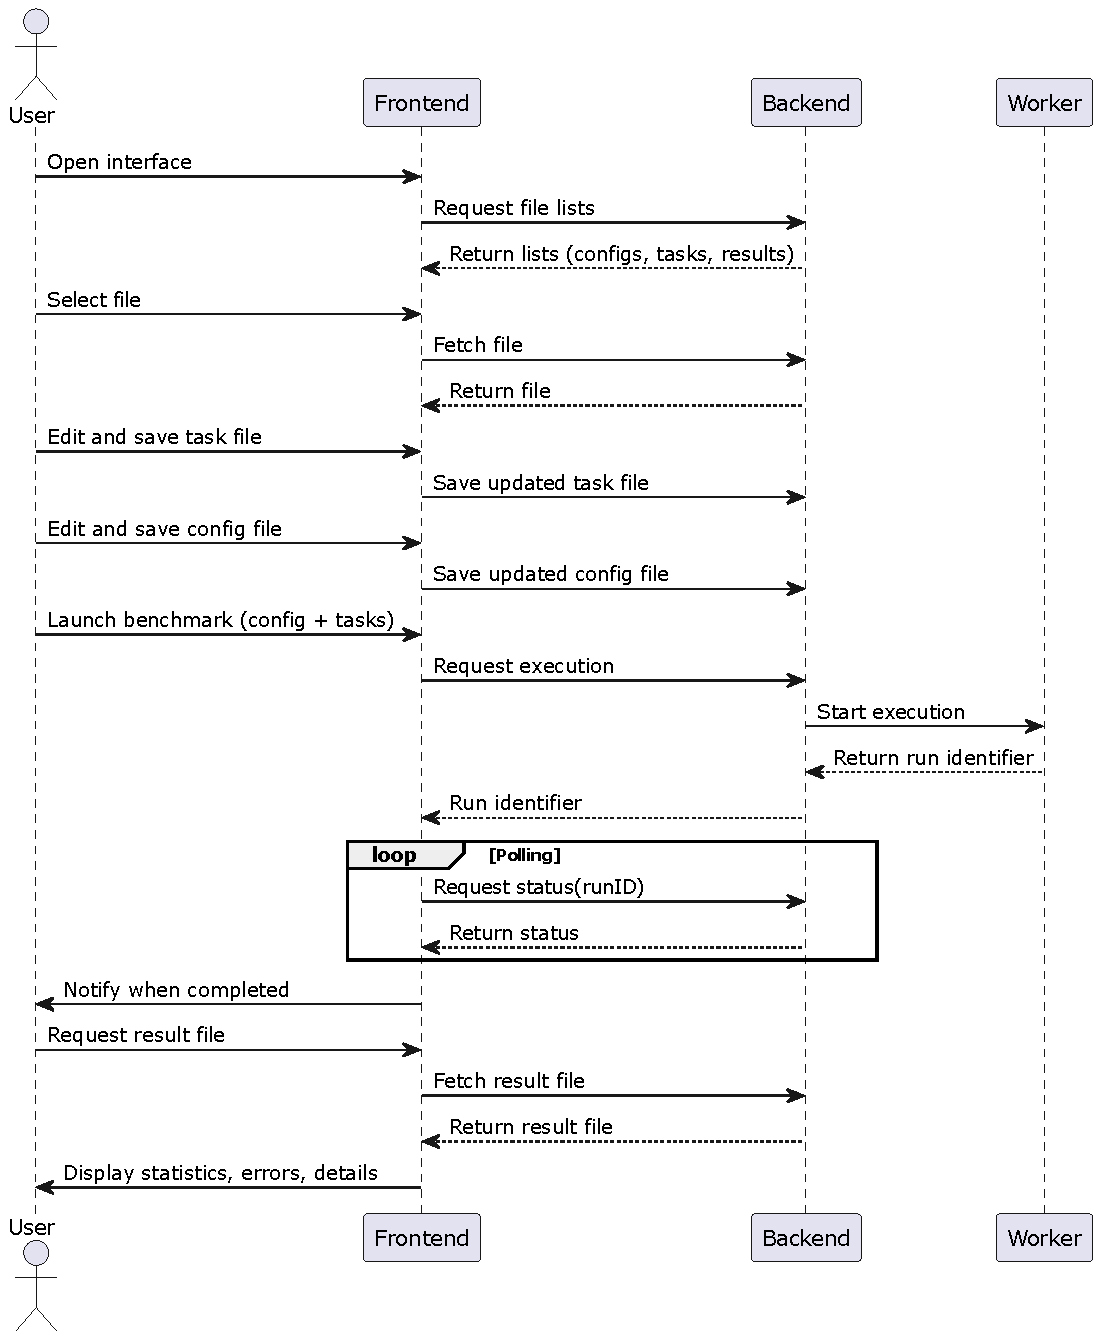
\includegraphics[width=0.9\textwidth]{./plantuml/sequence.pdf}
    \caption{Sequence Diagram.}
    \label{appendix:sequence}
\end{figure}

\chapter{User Interface Screenshots}
\label{appendix:ui_screenshots}

\begin{figure}[H]
    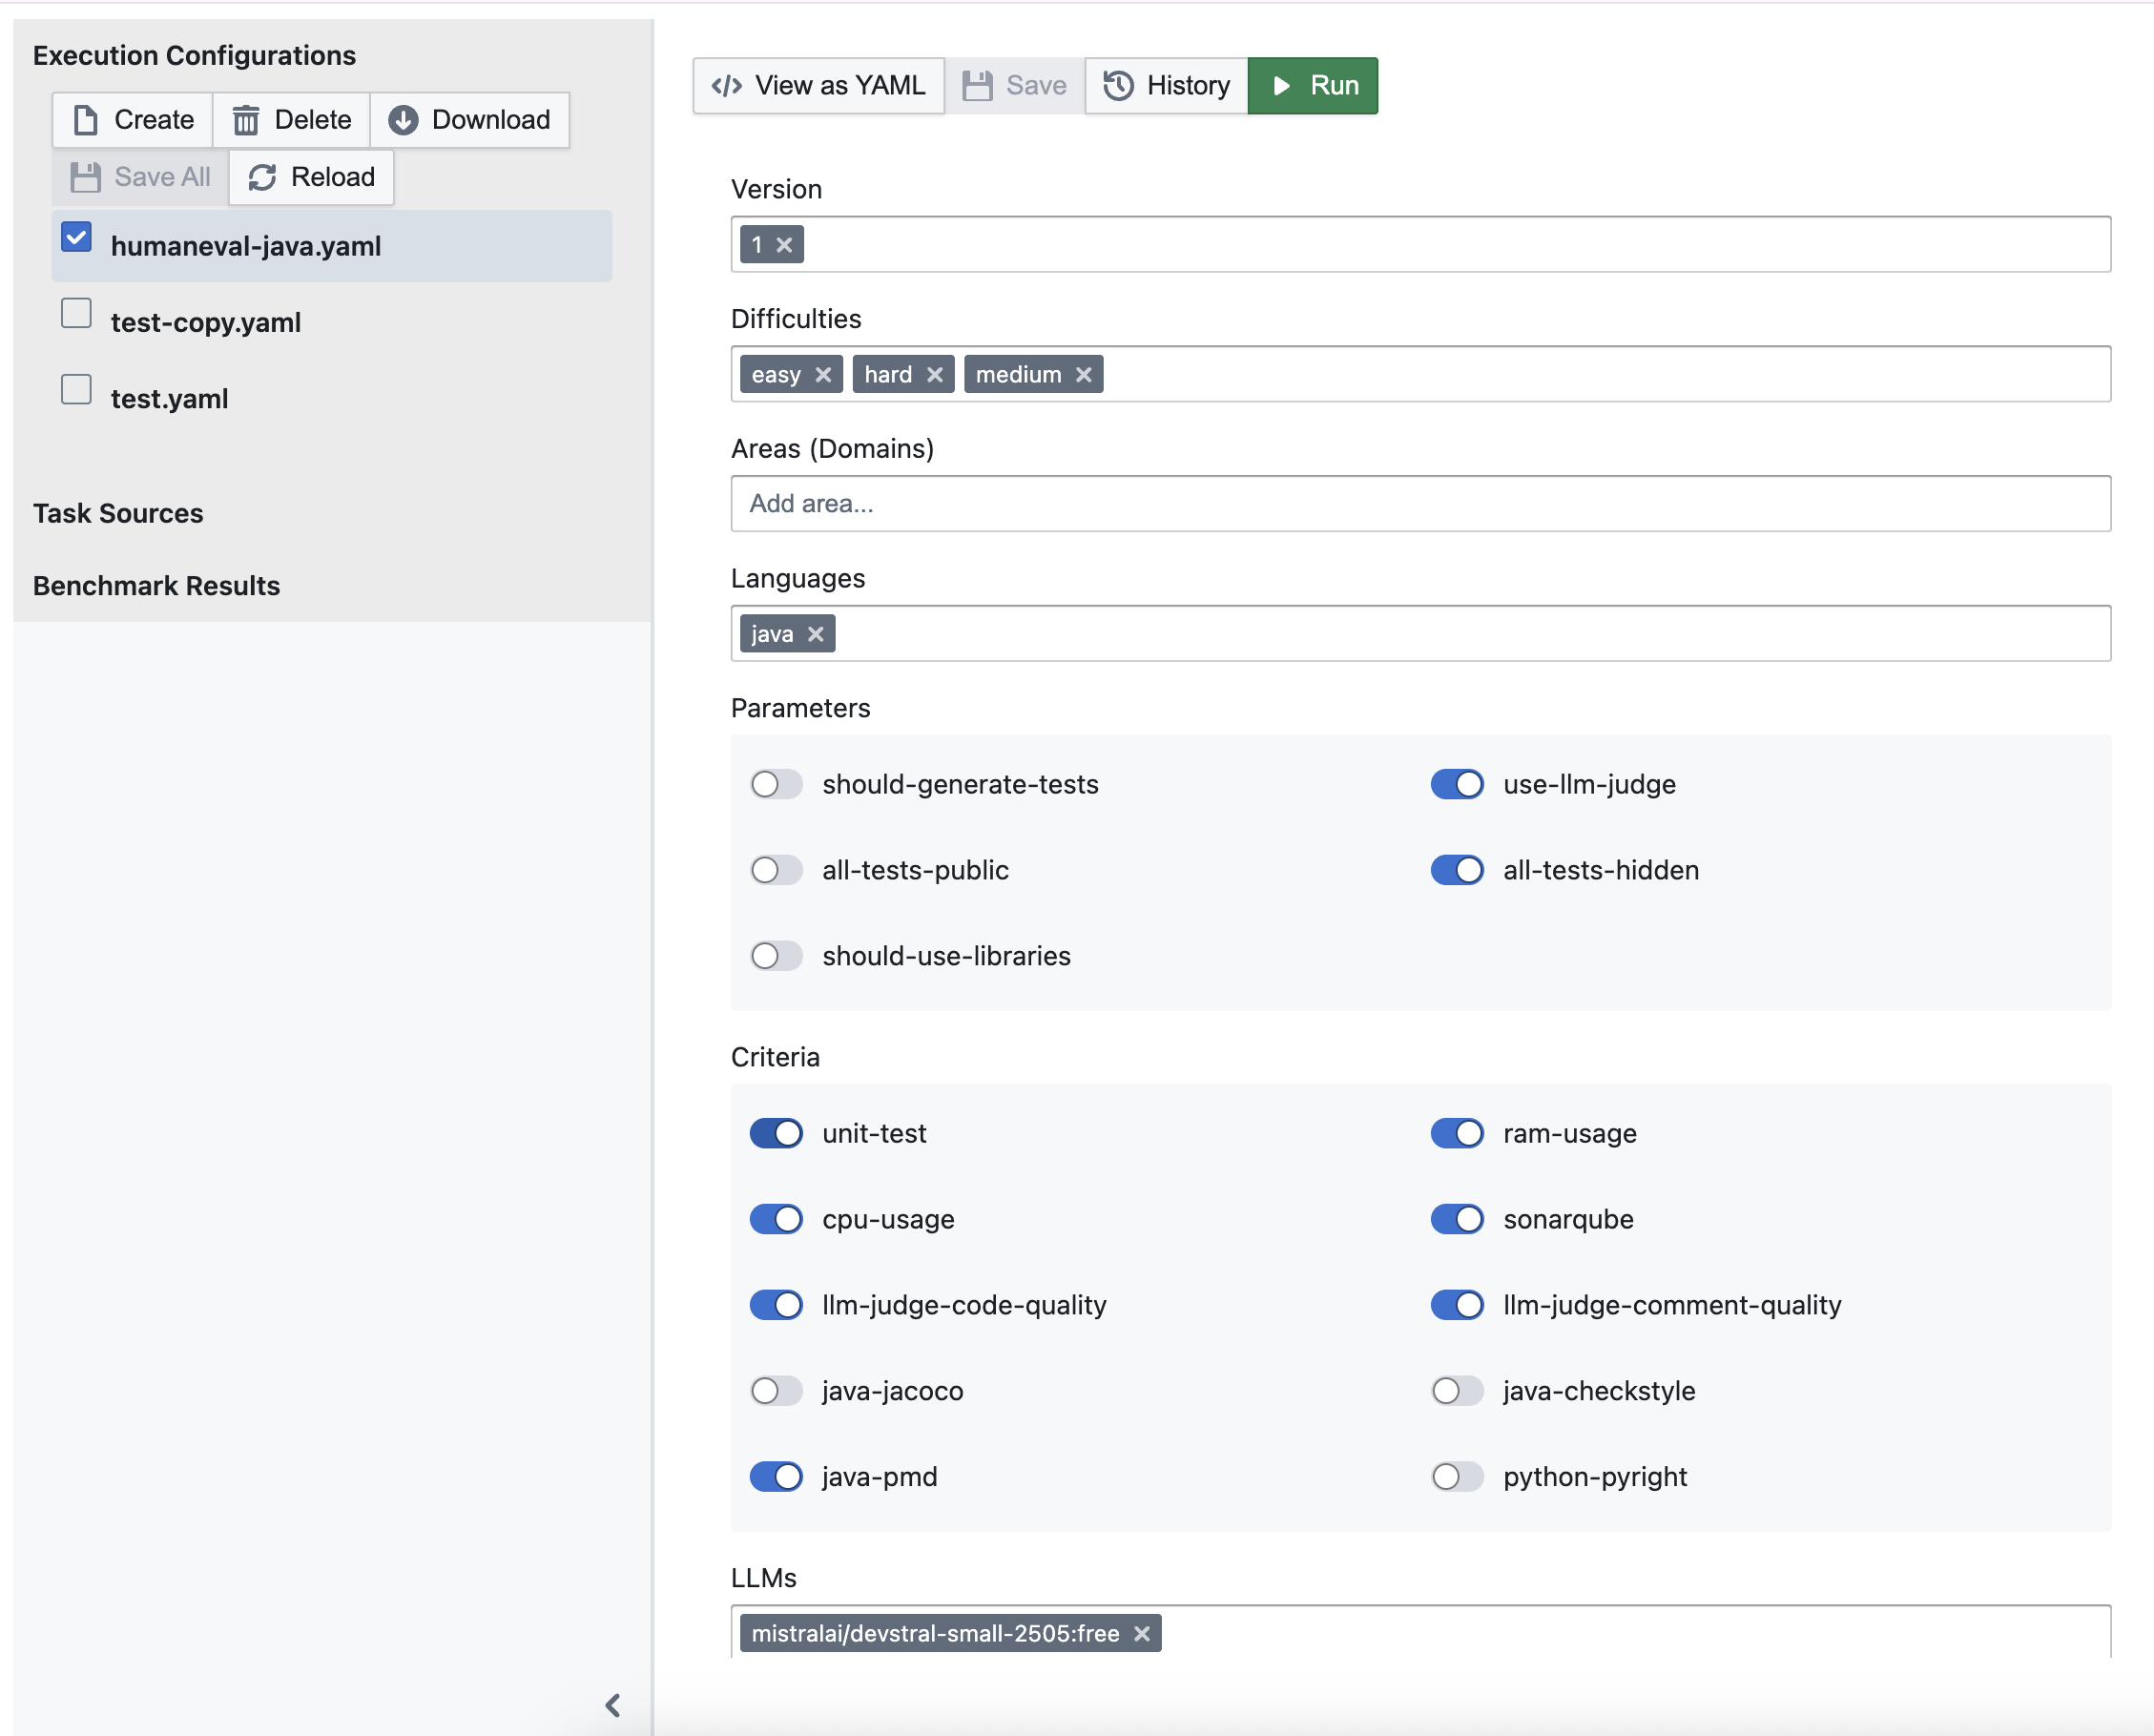
\includegraphics[width=0.9\textwidth]{./images/ui_exec_config}
    \caption{Execution Configuration visual editor.}
    \label{appendix:ui_exec_config}
\end{figure}


\begin{figure}[H]
    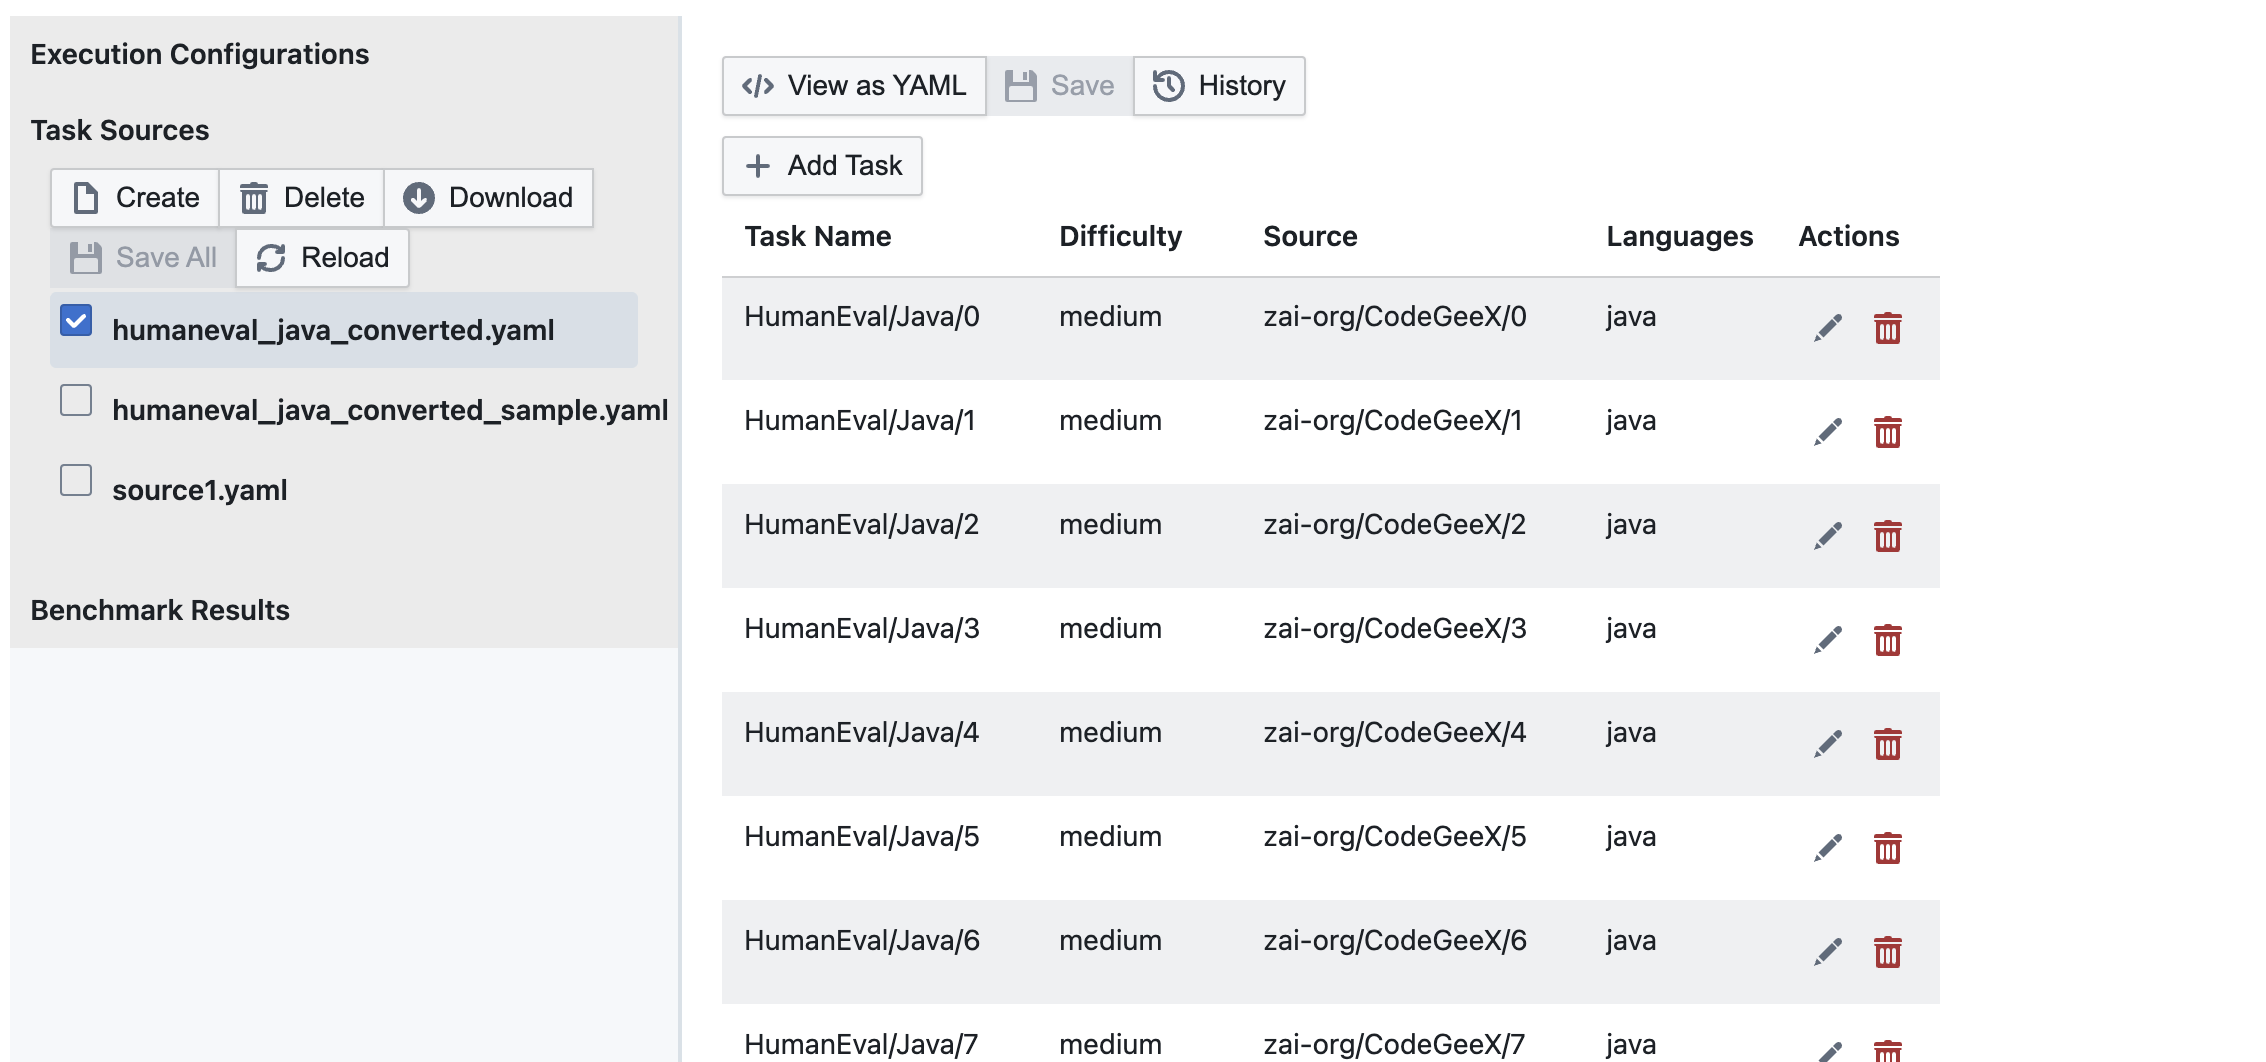
\includegraphics[width=0.9\textwidth]{./images/ui_task_source_list}
    \caption{Task Source visual editor. List of tasks in a Task Source.}
    \label{appendix:ui_task_source_list}
\end{figure}

\begin{figure}[H]
    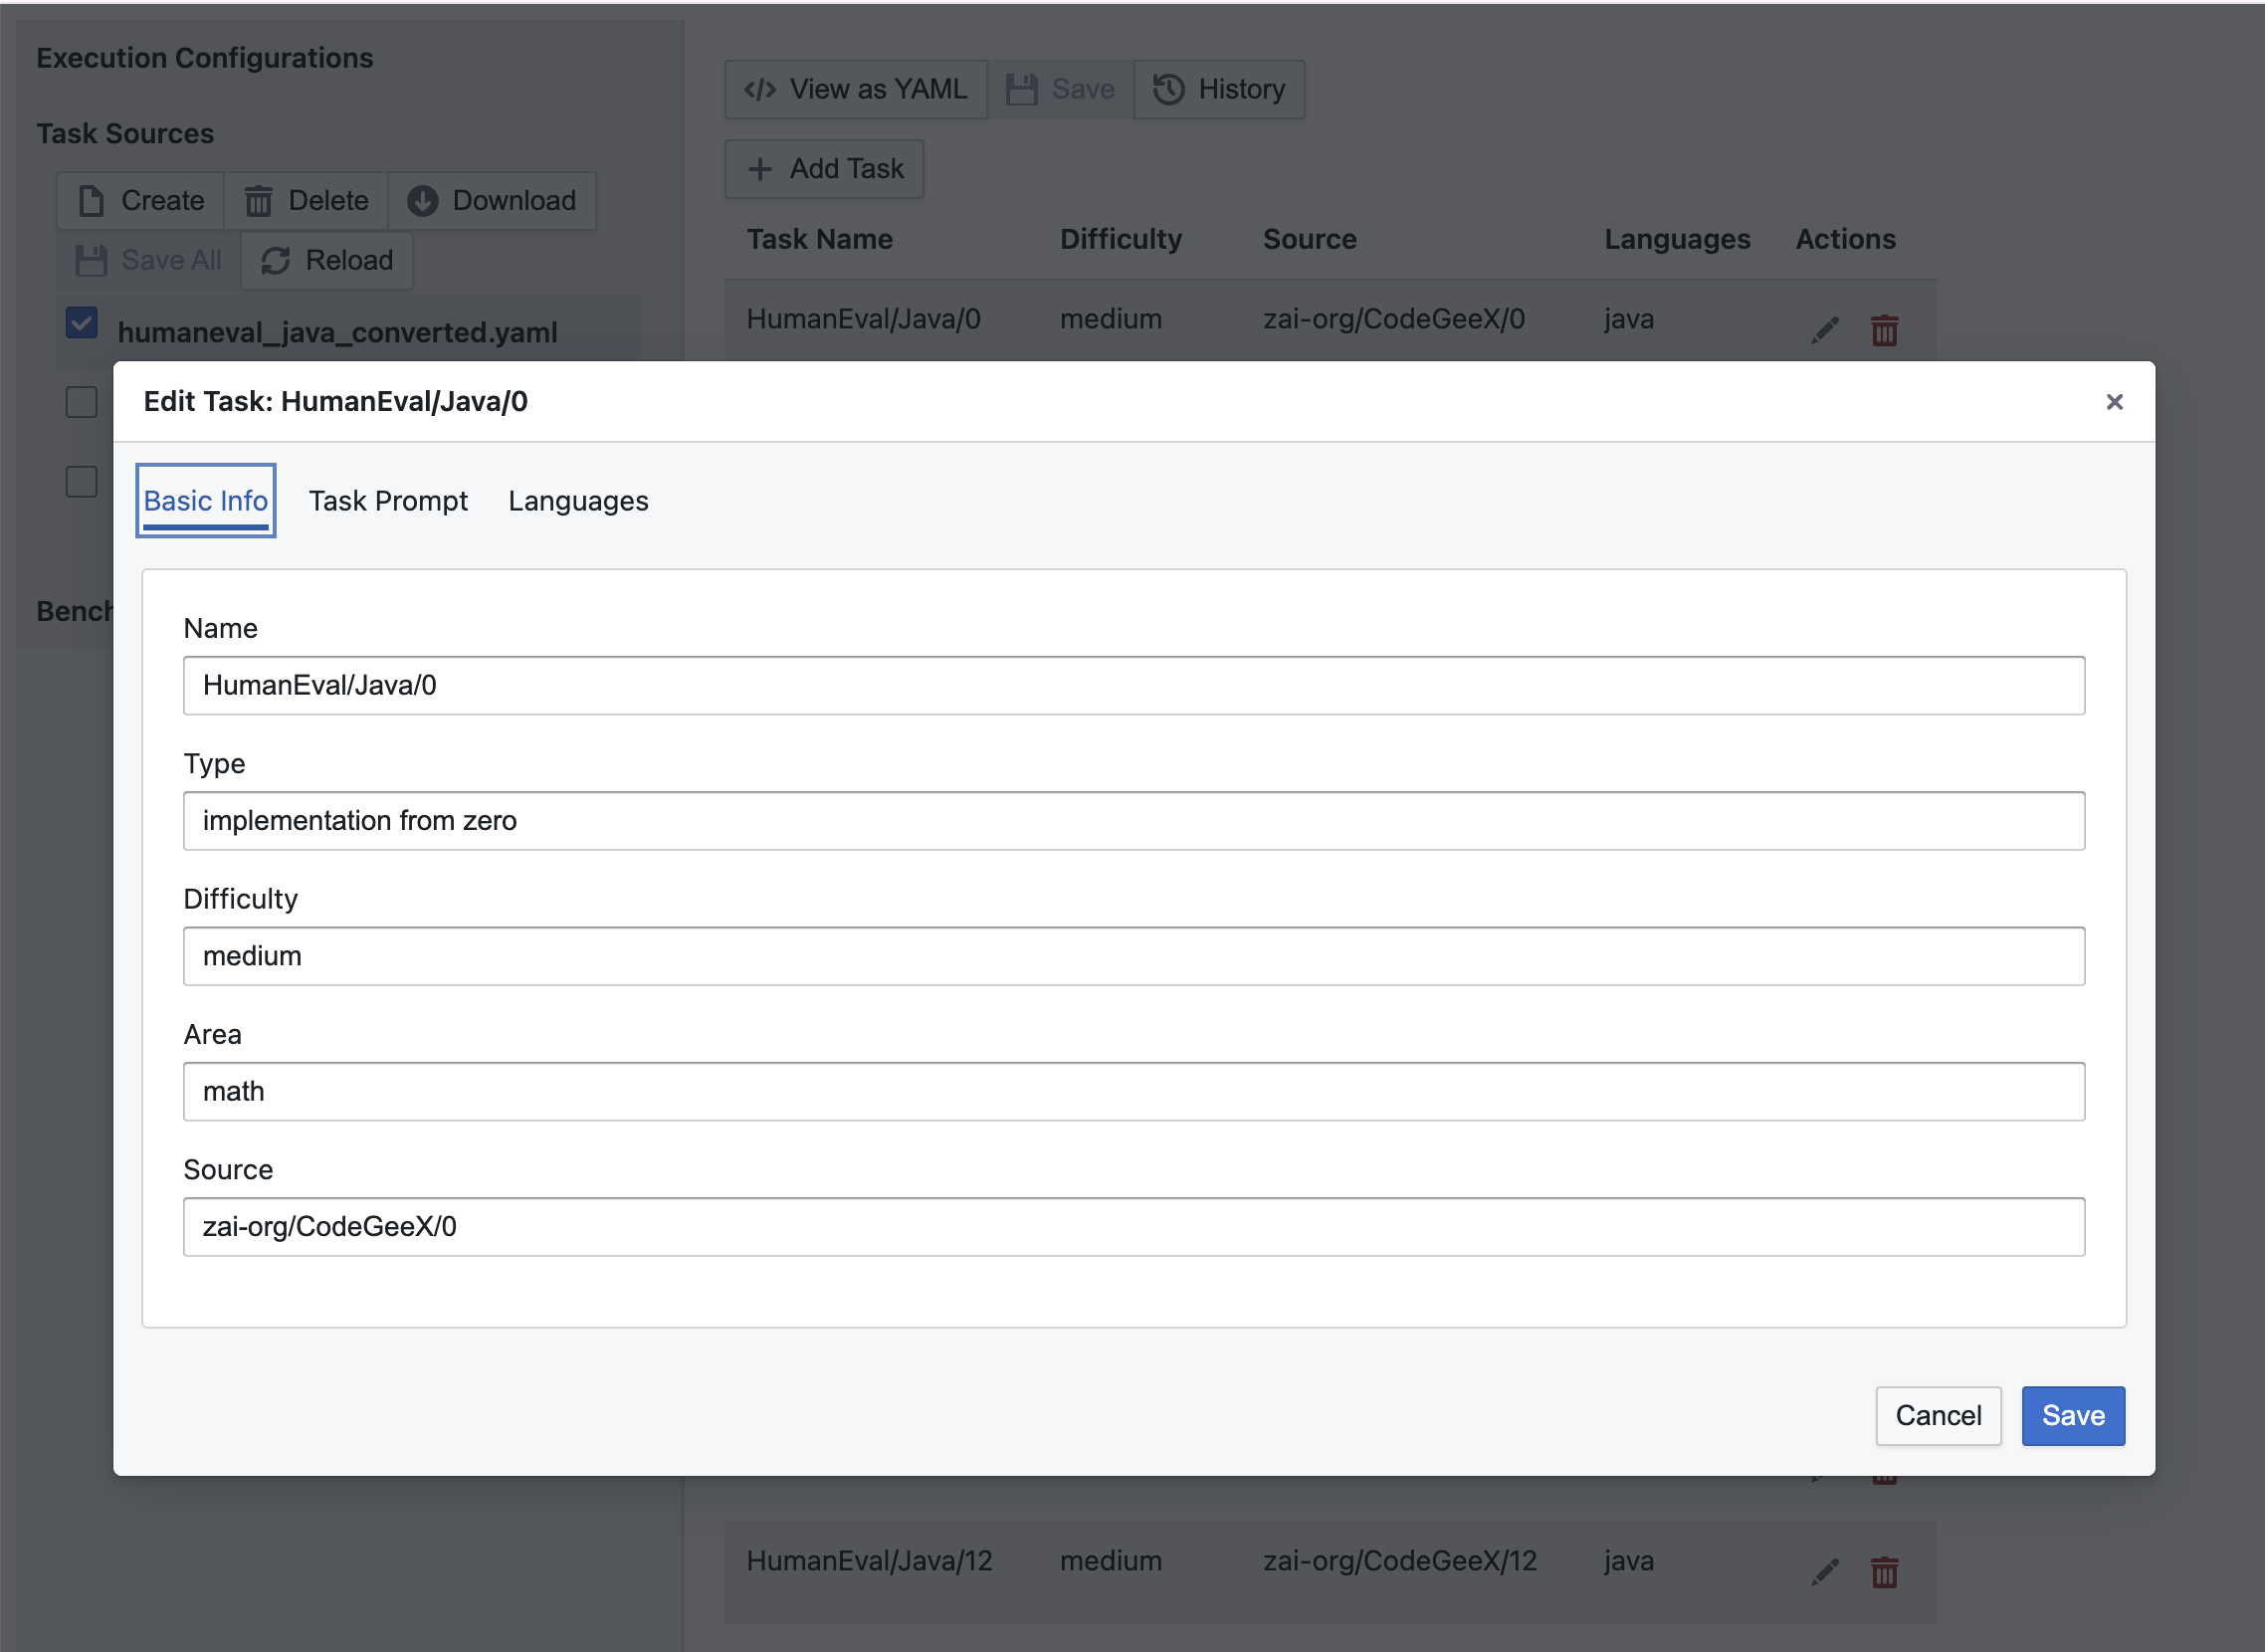
\includegraphics[width=0.9\textwidth]{./images/ui_task_source_info}
    \caption{Task Source visual editor. Basic information of a task.}
    \label{appendix:ui_task_source_info}
\end{figure}

\begin{figure}[H]
    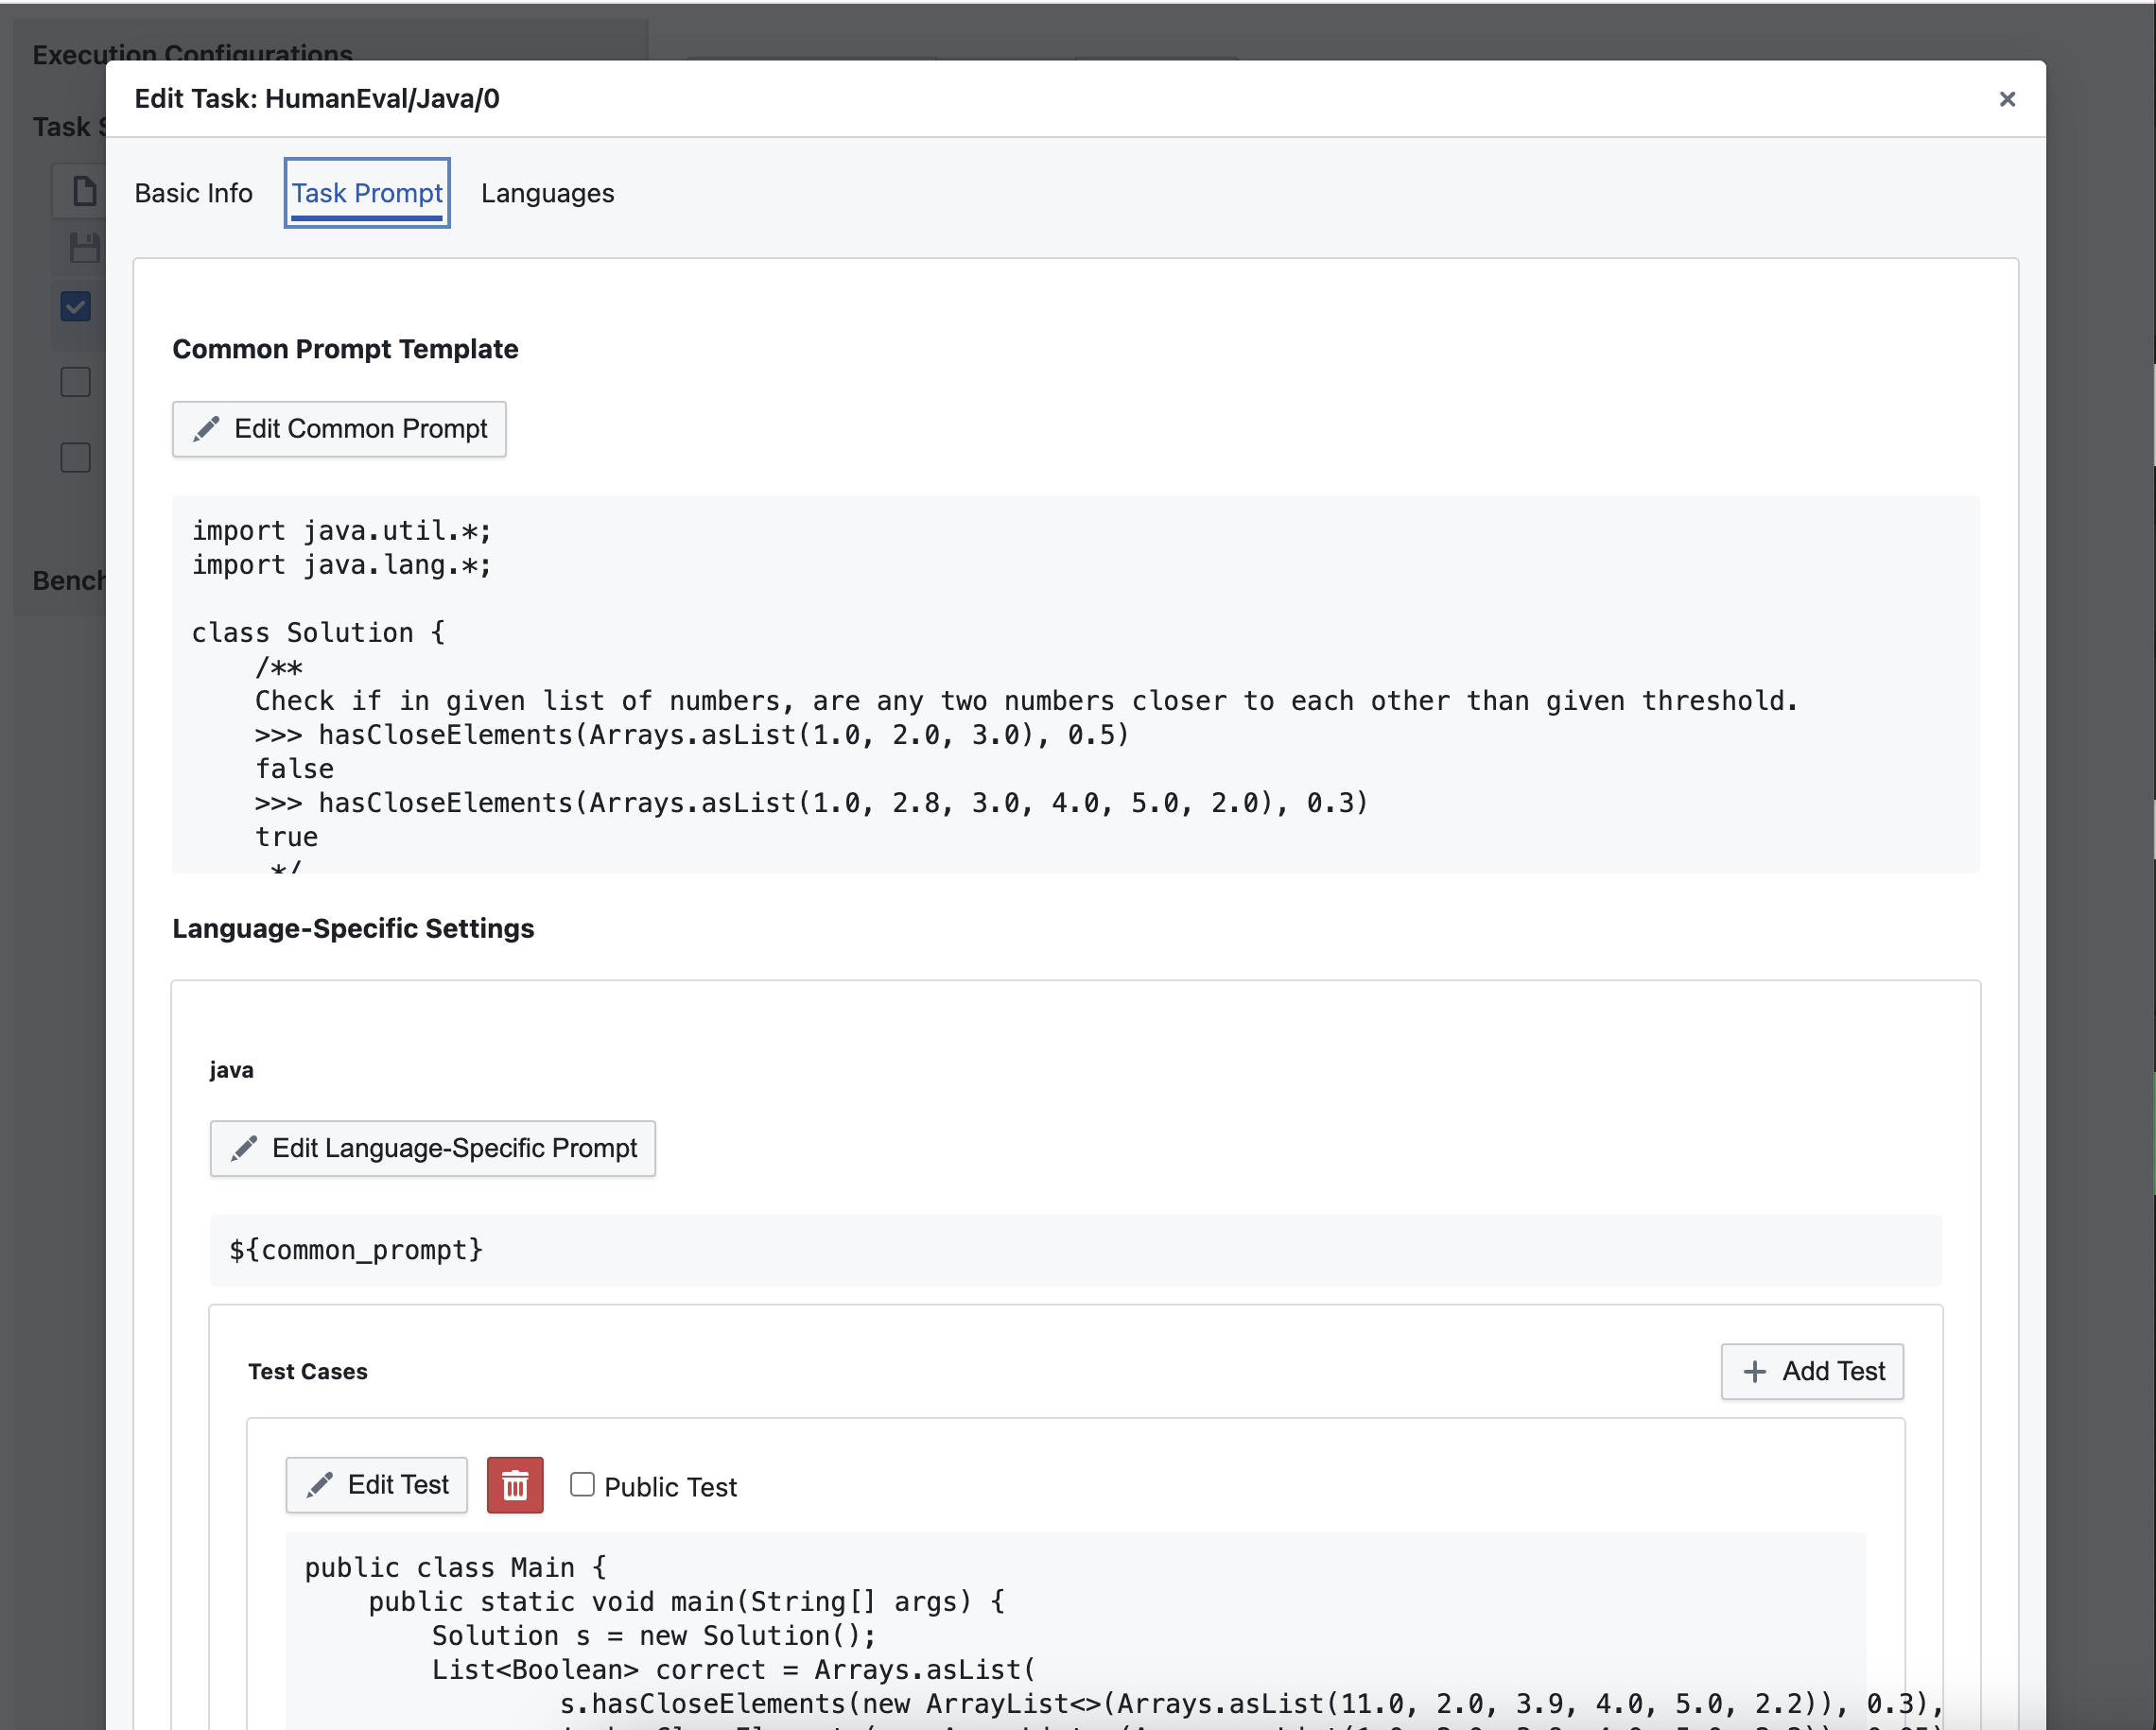
\includegraphics[width=0.9\textwidth]{./images/ui_task_source_prompts}
    \caption{Task Source visual editor. Prompts and tests of a task.}
    \label{appendix:ui_task_source_prompts}
\end{figure}

\begin{figure}[H]
    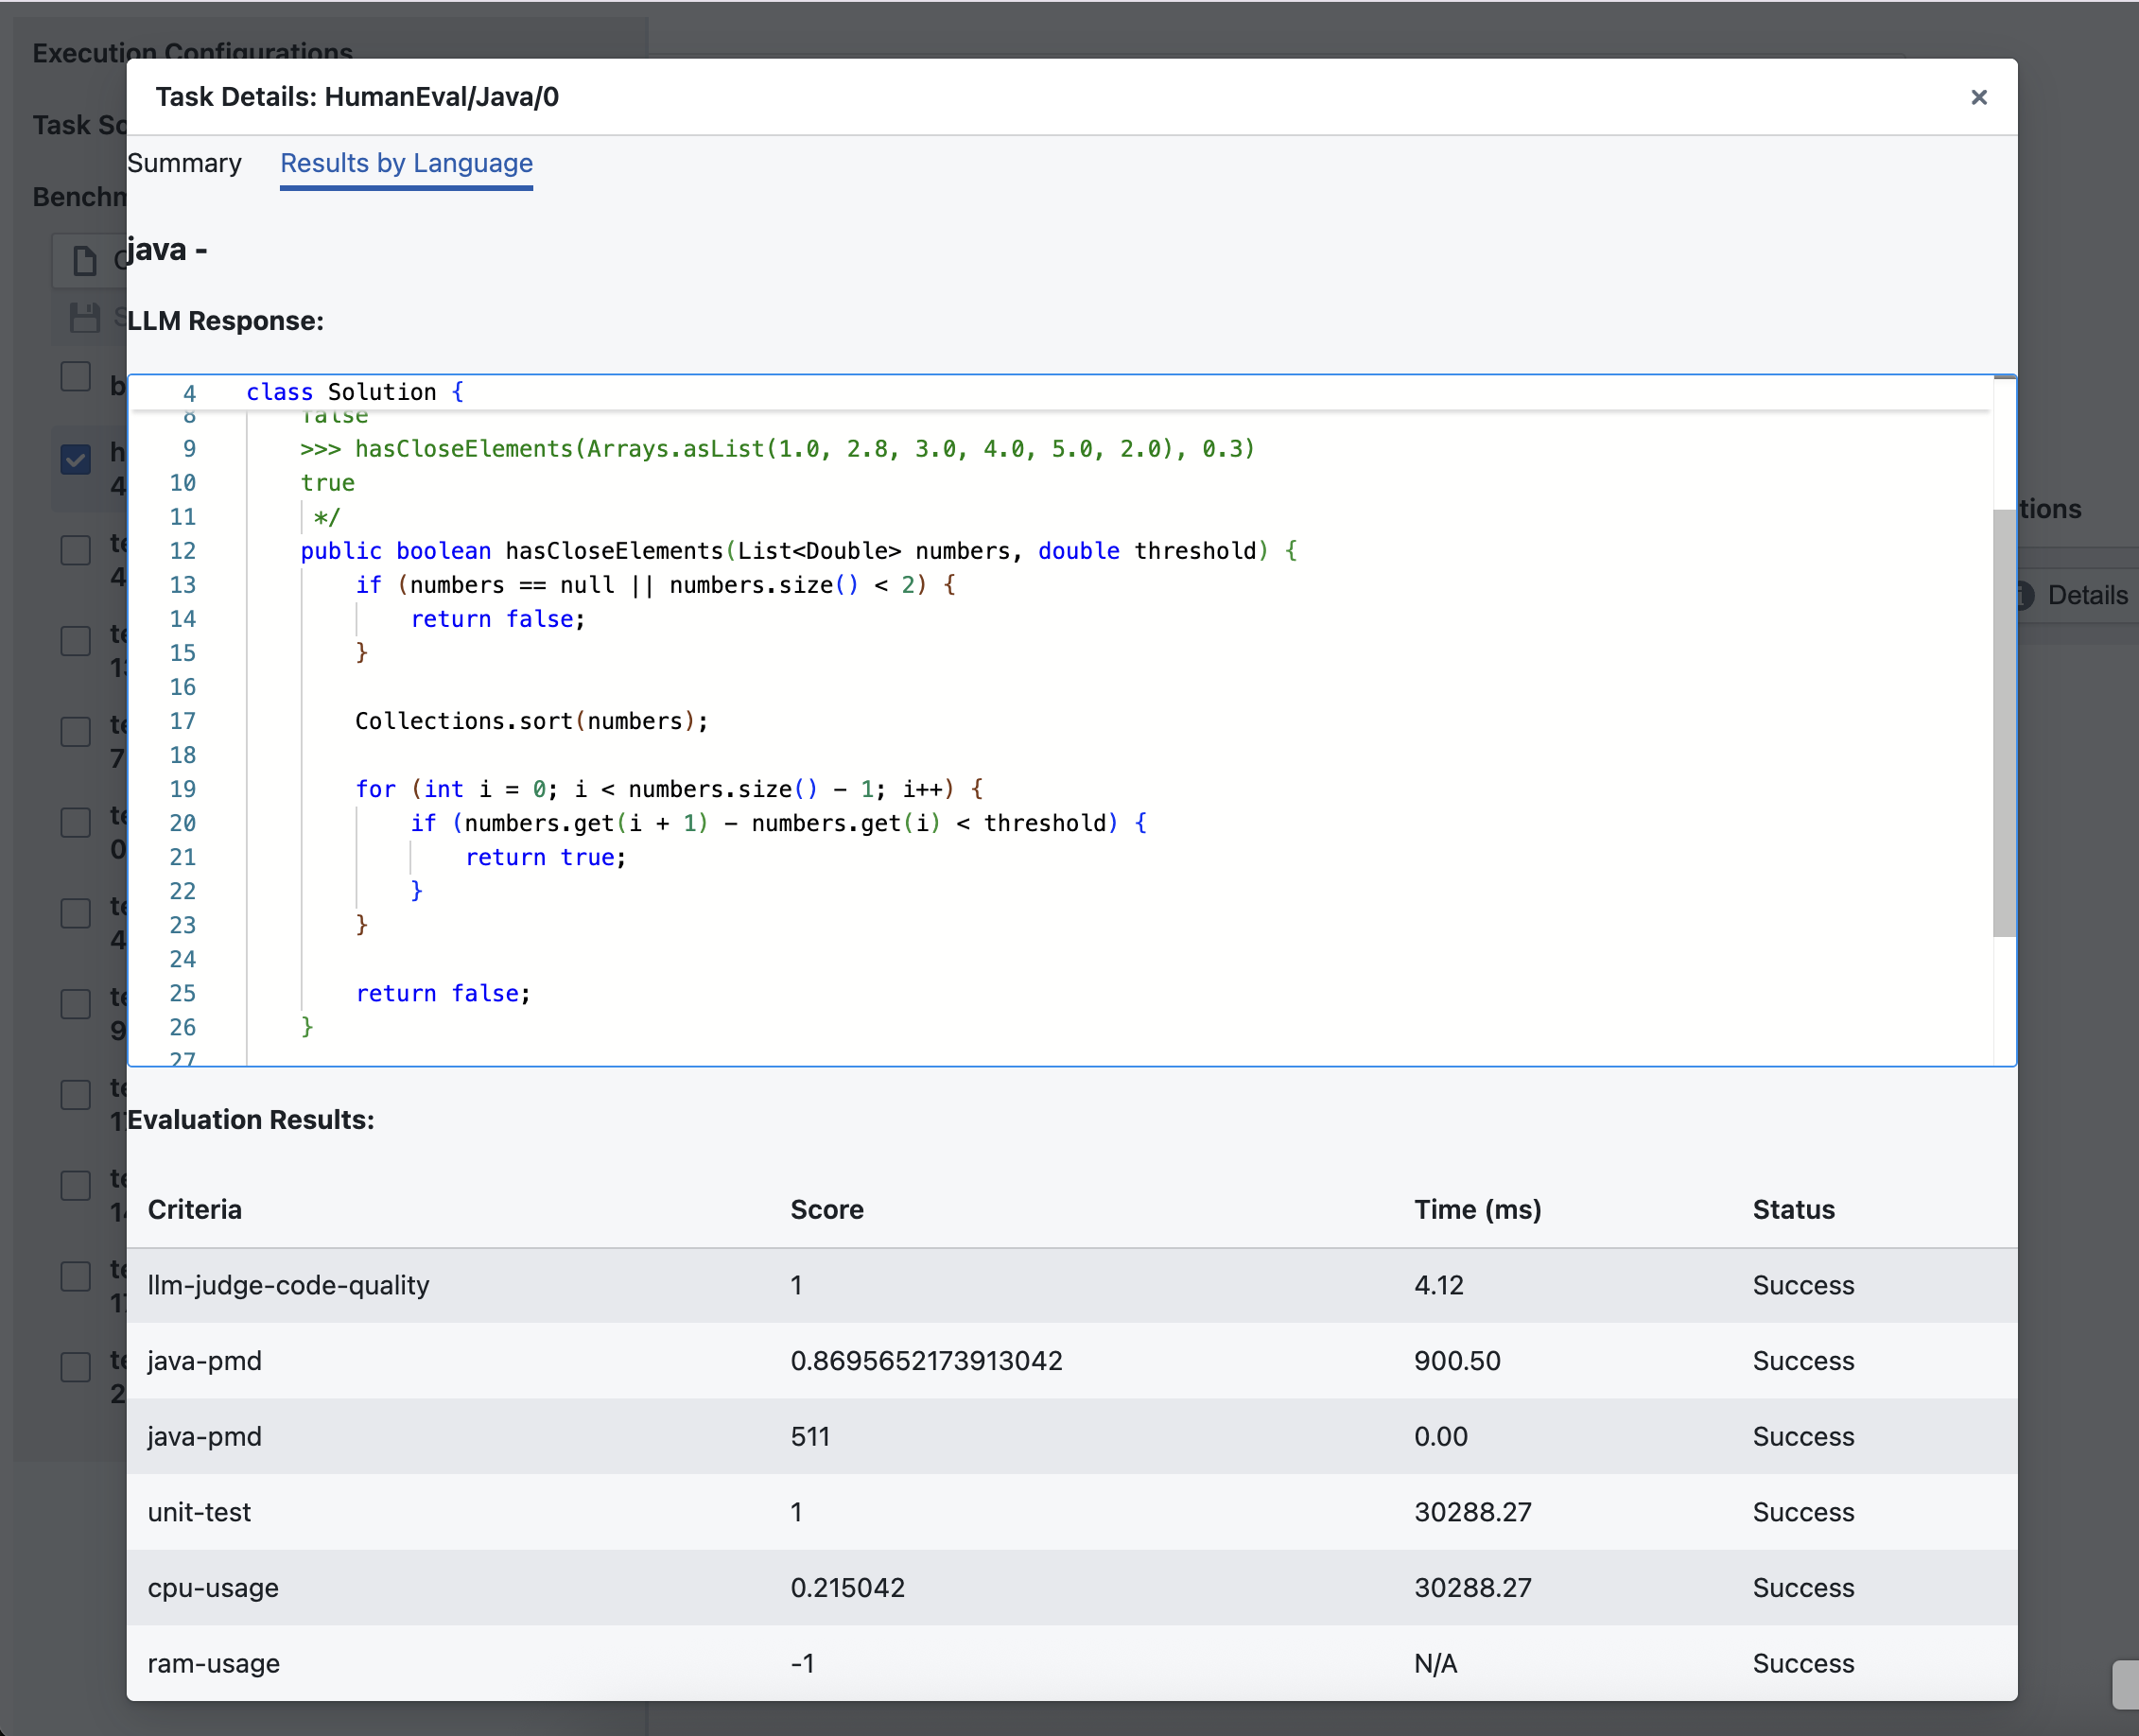
\includegraphics[width=0.9\textwidth]{./images/ui_result_single_task}
    \caption{Benchmark Results browser. }
    \label{appendix:ui_result_single_task}
\end{figure}

\chapter{Configuration and Result YAML Files}
\label{appendix:config_files}

TO-DO: Example of Configuration YAML file.

TO-DO: Example of Task Source YAML file.

TO-DO: Example of Benchmark Result YAML file.

TO-DO: Example of Benchmark Run Status YAML file.
    \end{appendices}
}{}


\end{document}